\PassOptionsToPackage{unicode=true}{hyperref} % options for packages loaded elsewhere
\PassOptionsToPackage{hyphens}{url}
%
\documentclass[]{article}
\usepackage{lmodern}
\usepackage{amssymb,amsmath}
\usepackage{ifxetex,ifluatex}
\usepackage{fixltx2e} % provides \textsubscript
\ifnum 0\ifxetex 1\fi\ifluatex 1\fi=0 % if pdftex
  \usepackage[T1]{fontenc}
  \usepackage[utf8]{inputenc}
  \usepackage{textcomp} % provides euro and other symbols
\else % if luatex or xelatex
  \usepackage{unicode-math}
  \defaultfontfeatures{Ligatures=TeX,Scale=MatchLowercase}
\fi
% use upquote if available, for straight quotes in verbatim environments
\IfFileExists{upquote.sty}{\usepackage{upquote}}{}
% use microtype if available
\IfFileExists{microtype.sty}{%
\usepackage[]{microtype}
\UseMicrotypeSet[protrusion]{basicmath} % disable protrusion for tt fonts
}{}
\IfFileExists{parskip.sty}{%
\usepackage{parskip}
}{% else
\setlength{\parindent}{0pt}
\setlength{\parskip}{6pt plus 2pt minus 1pt}
}
\usepackage{hyperref}
\hypersetup{
            pdftitle={Sea Stars of British Columbia},
            pdfauthor={Joan Moreaux},
            pdfborder={0 0 0},
            breaklinks=true}
\urlstyle{same}  % don't use monospace font for urls
\usepackage[margin=1in]{geometry}
\usepackage{graphicx,grffile}
\makeatletter
\def\maxwidth{\ifdim\Gin@nat@width>\linewidth\linewidth\else\Gin@nat@width\fi}
\def\maxheight{\ifdim\Gin@nat@height>\textheight\textheight\else\Gin@nat@height\fi}
\makeatother
% Scale images if necessary, so that they will not overflow the page
% margins by default, and it is still possible to overwrite the defaults
% using explicit options in \includegraphics[width, height, ...]{}
\setkeys{Gin}{width=\maxwidth,height=\maxheight,keepaspectratio}
\setlength{\emergencystretch}{3em}  % prevent overfull lines
\providecommand{\tightlist}{%
  \setlength{\itemsep}{0pt}\setlength{\parskip}{0pt}}
\setcounter{secnumdepth}{0}
% Redefines (sub)paragraphs to behave more like sections
\ifx\paragraph\undefined\else
\let\oldparagraph\paragraph
\renewcommand{\paragraph}[1]{\oldparagraph{#1}\mbox{}}
\fi
\ifx\subparagraph\undefined\else
\let\oldsubparagraph\subparagraph
\renewcommand{\subparagraph}[1]{\oldsubparagraph{#1}\mbox{}}
\fi

% set default figure placement to htbp
\makeatletter
\def\fps@figure{htbp}
\makeatother

\usepackage[font=small,format=plain,labelfont=bf,up,textfont=normal,up,justification=justified,singlelinecheck=false]{caption}
\usepackage{booktabs}
\usepackage{longtable}
\usepackage{array}
\usepackage{multirow}
\usepackage{wrapfig}
\usepackage{float}
\usepackage{colortbl}
\usepackage{pdflscape}
\usepackage{tabu}
\usepackage{threeparttable}
\usepackage{threeparttablex}
\usepackage[normalem]{ulem}
\usepackage{makecell}
\usepackage{xcolor}

\title{Sea Stars of British Columbia}
\author{Joan Moreaux}
\date{10/18/2021}

\begin{document}
\maketitle

\hypertarget{sea-stars-of-bamfield-bc}{%
\section{Sea Stars of Bamfield, BC}\label{sea-stars-of-bamfield-bc}}

\hypertarget{pisaster-ochraceus}{%
\subsection{Pisaster ochraceus:}\label{pisaster-ochraceus}}

\hypertarget{description}{%
\subsubsection{Description}\label{description}}

Written description: Pisaster ochraceus, known commonly as the Ochre
Star, has five rays that taper towards the end and a prominent network
of white spines (Brietzke et al., 2013). It can be purple, orange,
yellow, or brown, and has a very stiff body. It is commonly confused
with Evasterias troschelii, but can be differentiated by its large
central disk and shorter, thicker rays (Harbo, 2011).

Questions:

Paragraph description: \textbf{Range and Habitat:} \emph{P. ochraceus}
is found from Alaska to California (Brietzke et \emph{al.}, 2013), and
is very abundant on the West Coast of British Columbia. The Ochre Star
is found in the mid-to-low intertidal, but can also be found subtidally
to a depth of 88m (McFadden et \emph{al.}, 2008). It prefers living on
rocks or mussel beds; juveniles can also be found under rocks (Brietzke
et \emph{al.}, 2013). The species suffered from a mass mortality event
along the West Coast of North America in 2017 because of the spread of
the sea star wasting disease (B.C. Coast Edition, 2018).

\textbf{Trophic Role:} \emph{P. ochraceus} is the apex predator of the
intertidal, as it is rarely preyed upon. Occasionally, sea otters or
seagulls may eat sea stars (Multi-Agency Rocky Intertidal Network,
2021). The species mainly feeds on mussels, but can also prey on
barnacles, limpets and snails (Brietzke et \emph{al.}, 2013). \emph{P.
ochraceus}, like many other species in the class Asteroidea, feed by
everting their stomach out of their body and around their prey, to start
external digestion (McFadden et \emph{al.}, 2008).

\hypertarget{eubalaena-australis-southern-right-whale}{%
\section{\texorpdfstring{\emph{Eubalaena australis} (Southern right
whale)}{Eubalaena australis (Southern right whale)}}\label{eubalaena-australis-southern-right-whale}}

\hypertarget{description-1}{%
\subsection{Description}\label{description-1}}

These stocky whales have extremely large heads, which can be over
one-fourth of the body length. The mouthline is bowed and the rostrum is
arched. Text text text text. \textbf{Bold text bold text bold text.}
\emph{Italicized text italicized text italicized text}. Text text text
text. \textbf{Bold text bold text bold text.} \emph{Italicized text
italicized text italicized text}. Text text text text. \textbf{Bold text
bold text bold text.} \emph{Italicized text italicized text italicized
text}. Text text text text. \textbf{Bold text bold text bold text.}
\emph{Italicized text italicized text italicized text}. Text text text
text. \textbf{Bold text bold text bold text.} \emph{Italicized text
italicized text italicized text}. Text text text text. \textbf{Bold text
bold text bold text.} \emph{Italicized text italicized text italicized
text}. Text text text text. \textbf{Bold text bold text bold text.}
\emph{Italicized text italicized text italicized text}. Text text text
text. \textbf{Bold text bold text bold text.} \emph{Italicized text
italicized text italicized text}. Text text text text. \textbf{Bold text
bold text bold text.} \emph{Italicized text italicized text italicized
text}. Text text text text. \textbf{Bold text bold text bold text.}
\emph{Italicized text italicized text italicized text}. Text text text
text. \textbf{Bold text bold text bold text.} \emph{Italicized text
italicized text italicized text}.

\newpage

\hypertarget{figures}{%
\subsection{Figures}\label{figures}}

\begin{figure}

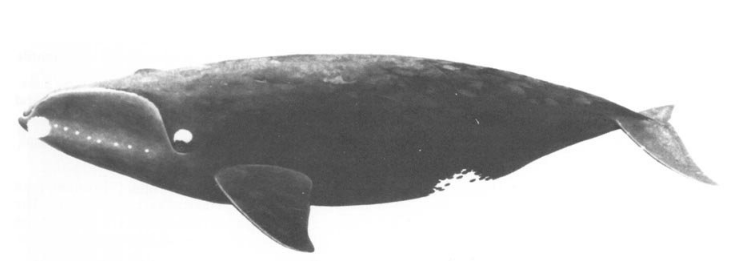
\includegraphics[width=0.5\linewidth,height=0.3\textheight]{/Users/joanmoreaux/Github/species-id-starfish/images/southern-right} \hfill{}

\caption{This is the southern right whale, figure is centered.}\label{fig:southern-right-whale}
\end{figure}

\begin{figure}

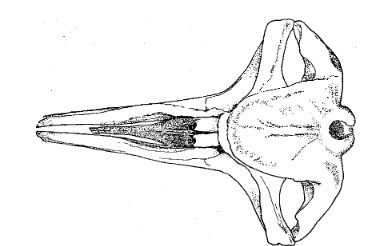
\includegraphics[width=0.5\linewidth,height=0.3\textheight]{/Users/joanmoreaux/Github/species-id-starfish/images/southern-right-skull} \hfill{}

\caption{This is the skull of the southern right whale skull (dorsal view), figure is left-aligned.}\label{fig:southern-right-whale-skull}
\end{figure}

\begin{figure}

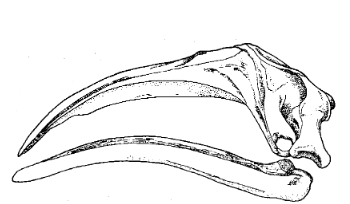
\includegraphics[width=0.5\linewidth,height=0.3\textheight]{/Users/joanmoreaux/Github/species-id-starfish/images/southern-right-skull-lateral} \hfill{}

\caption{This is the skull of the southern right whale skull (lateral view), figure is left-aligned.}\label{fig:southern-right-whale-skull-lateral}
\end{figure}

\newpage

\hypertarget{questions}{%
\subsection{Questions}\label{questions}}

\begin{enumerate}
\def\labelenumi{\arabic{enumi}.}
\tightlist
\item
  Very interesting and useful question
\item
  Another wildly helpful question
\item
  A third, MOST fascinating question
\end{enumerate}

\hypertarget{balaena-mysticetus-bowhead-whale}{%
\section{\texorpdfstring{\emph{Balaena mysticetus} (Bowhead
whale)}{Balaena mysticetus (Bowhead whale)}}\label{balaena-mysticetus-bowhead-whale}}

\hypertarget{description-2}{%
\subsection{Description}\label{description-2}}

Bowhead whales are very rotund, but often have a distinct ``neck''
region. The head is large\ldots{} Text text text text. \textbf{Bold text
bold text bold text.} \emph{Italicized text italicized text italicized
text}. Text text text text. \textbf{Bold text bold text bold text.}
\emph{Italicized text italicized text italicized text}. Text text text
text. \textbf{Bold text bold text bold text.} \emph{Italicized text
italicized text italicized text}. Text text text text. \textbf{Bold text
bold text bold text.} \emph{Italicized text italicized text italicized
text}. Text text text text. \textbf{Bold text bold text bold text.}
\emph{Italicized text italicized text italicized text}. Text text text
text. \textbf{Bold text bold text bold text.} \emph{Italicized text
italicized text italicized text}. Text text text text. \textbf{Bold text
bold text bold text.} \emph{Italicized text italicized text italicized
text}. Text text text text. \textbf{Bold text bold text bold text.}
\emph{Italicized text italicized text italicized text}. Text text text
text. \textbf{Bold text bold text bold text.} \emph{Italicized text
italicized text italicized text}. Text text text text. \textbf{Bold text
bold text bold text.} \emph{Italicized text italicized text italicized
text}. Text text text text. \textbf{Bold text bold text bold text.}
\emph{Italicized text italicized text italicized text}. Text text text
text. \textbf{Bold text bold text bold text.} \emph{Italicized text
italicized text italicized text}.

\newpage

\hypertarget{figures-1}{%
\subsection{Figures}\label{figures-1}}

\begin{figure}
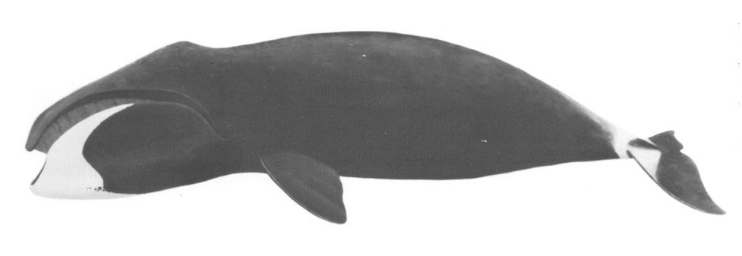
\includegraphics[width=0.5\linewidth,height=0.3\textheight]{/Users/joanmoreaux/Github/species-id-starfish/images/bowhead} \caption{This is the bowhead whale, figure is centered.}\label{fig:bowhead-whale}
\end{figure}

\begin{figure}
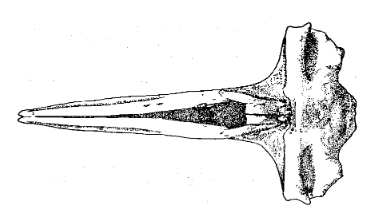
\includegraphics[width=0.5\linewidth,height=0.3\textheight]{/Users/joanmoreaux/Github/species-id-starfish/images/bowhead-skull} \caption{This is the skull of the bowhead whale skull, figure is centered.}\label{fig:bowhead-whale-skull}
\end{figure}

\begin{figure}
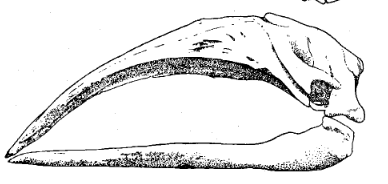
\includegraphics[width=0.5\linewidth,height=0.3\textheight]{/Users/joanmoreaux/Github/species-id-starfish/images/bowhead-skull-lateral} \caption{This is the skull of the bowhead whale skull, figure is centered.}\label{fig:bowhead-whale-skull-lateral}
\end{figure}

\newpage

\hypertarget{questions-1}{%
\subsection{Questions}\label{questions-1}}

\begin{enumerate}
\def\labelenumi{\arabic{enumi}.}
\tightlist
\item
  Very interesting and useful question
\item
  Another wildly helpful question
\item
  A third, MOST fascinating question
\end{enumerate}

\newpage

\hypertarget{supplemental-information}{%
\section{Supplemental Information}\label{supplemental-information}}

\begin{tabular}{lllll}
\toprule
Species & Max.Size..diameter. & Morphology & Trophic.Role & Reproductive.Mode\\
\midrule
Pisaster ochraceus & 50 cm & \makecell[l]{Very polymorphic in colour (commonly purple or orange)\\\\Long rays which are widest at base\\\\Typically five rays\\\\Stellate patterned ossicles on central disk of aboral surface\\\\Prominent white spines} & \makecell[l]{Key stone species\\\\Prey: mussels, barnacles, limpets, and snails\\\\Feeding mechanism: external digestion via stomach eversion\\\\Predators: seagulls, otters} & \makecell[l]{Assexual (fission)\\\\Sexual through external fertilization (May & July)\\\\Free living ciliated bipinnaria larvae}\\
Evasterias troschelii & 80cm & \makecell[c]{Polymorphic in colour, commonly brown, orange, or blue-grey\\\\Slender long rays which are widest shortly after base of ray\\\\Typically five rays\\\\Netlike or pentagonal patterned ossicles on aboral surface\\\\Few white spines} & \makecell[c]{Prey: **bivalves, barnacles**, tunicates, chitons, and other sea stars\\\\Predators: Sea stars and Alaska King Crab} & \makecell[c]{Assexual (fission)\\\\Free living ciliated bipinnaria larvae}\\
Patiria miniata & 25cm & \makecell[r]{Extremely variable colour; can be red, blue, yellow, green, brown, and solid or patterned\\\\Rays are short and broad \\\\Webbed tissue between rays\\\\Typically 5-6 rays (can have 3-8)\\\\Flat crescent shaped ossicles on aboral surface} & \makecell[r]{Omnivore and scavenger\\\\Prey: sea stars, tunicates, algae, and decaying organisms\\\\Feeding mechanism: external digestion via stomach eversion\\\\Predators: molluscs, crustaceans, and sea stars\\\\Predator deterrent: chemical defense} & \makecell[r]{Assexual (fission)\\\\Sexual through external fertilization (especially in late winter or spring)\\\\Free living ciliated bipinnaria larvae}\\
Dermasterias imbricata & 30 cm & \makecell[l]{Grey, yellow, or red, with patches of red, brown, purple\\\\Rays are short and broad\\\\Typically five rays (can have six or seven)\\\\Ossicles are absent leaving a smooth or leathery surface\\\\May have the scent of garlic} & \makecell[l]{Prey: **Sea anemone**, sea cucumbers, sea urchins sea sponges, chitons\\\\Feeding mechanism: swallows prey and digests\\\\Predators: sea otters\\\\Predator deterrent: Garlic smelling chemical} & \makecell[l]{Assexual (fission)\\\\Sexual through external fertilization (April-August)\\\\Free living ciliated bipinnaria larvae}\\
\bottomrule
\end{tabular}

\hypertarget{supplemental-information-1}{%
\section{Supplemental Information}\label{supplemental-information-1}}

\begin{table}

\caption{\label{tab:unnamed-chunk-2}Whale morphometrics and other infomration.}
\centering
\begin{tabular}[t]{l|l|l|l|l|l}
\hline
Species & Length & Weight & Trophic Role & Diet & Reproduction\\
\hline
Bowhead whale & 18..7-20.8 & 81542.79 - 90700 & predators & kril & sexual\\
\hline
Southern right whale & 14.5-18.2 & 63576.92 - 79800 & predators & krill & sexual\\
\hline
\end{tabular}
\end{table}

\hypertarget{figures-2}{%
\subsection{Figures}\label{figures-2}}

\begin{figure}
\includegraphics[width=0.5\linewidth,height=0.5\textheight]{guide-template_files/figure-latex/unnamed-chunk-3-1} \caption{Whale length and whale weight compared by species}\label{fig:unnamed-chunk-3}
\end{figure}

\end{document}
